\chapter{Curve fitting of potential for MMO without photoemission}
\label{sec:second-app}
\newenvironment{longlisting}{\captionsetup{type=listing}}{}

From \cref{sec:results} it became apparent from the timeseries plot of the potential of the MMO spacecraft in the cases where photoemission was not included that a convergence to a floating potential had not been achieved. In this appendix we present a Python script for fitting curves to these timeseries plots of potential in order to estimate the floating potential that PINC would eventually converge to.

Three functions were optimized to fit against the absolute value of the potential and compared for accuracy.
\begin{subequations}
    \begin{align}
        \text{Hill function:} \: y(t) &= \frac{x}{h + t}\label{eq:Hill} \\
        \text{Exponential function:} \: y(t) &= a \exp{-b t} - c \label{eq:expFit} \\
        \text{Generalized logistic function} \: y(t) &=  A + \frac{K - A}{\left(C + Q e^{-B t}\right)^{\frac{1}{\nu}}}.\label{eq:genLog}
    \end{align}
\end{subequations}
The three functions described all converge to a finite value, and the rate of growth can be easily controlled. The function parameters, except the independent variable $t$ denoting time, are constants and can be adjusted for optimum fit. The Python package Scipy contains a curve fitting function. This curve fitting function uses a non-linear least squares algorithm to fit some function to a data set. This was combined with a trial and error checking of parameters since the optimization function did not converge for the exponential and generalized logistic function when all the controllable parameters were included. 

The python script below also outputs the root mean square error, such that the fit of our trial functions could be tested during trial and error testing. The root mean square error is described as:
\begin{equation}\label{eq:RMSE}
    \text{RMSE} = \sqrt{\frac{\sum^n_{i=1} \left(y_{pred,i} - y_i \right)^2}{n}}
\end{equation}

The absolute value of the potential found with PINC simulation was used to simplify fitting the trial functions to the data, the independent time variable $t$ was also normalized by 10,000 timesteps to reduce errors from small floating point operations when computing the $e^{-b t}$ term found in two of the trial functions.
\begin{center}
\begin{figure}[H]
  \begin{subfigure}[b]{0.61\textwidth}
    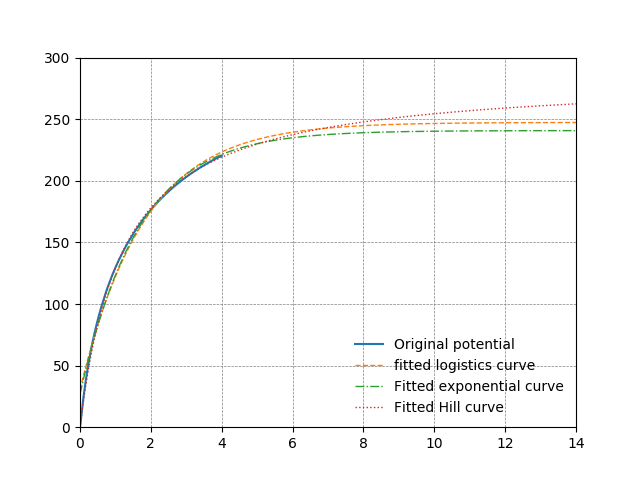
\includegraphics[width=\textwidth]{figures/Appendix/C_fit_NB.png}
    \caption{14,000 timesteps}
    \label{fig:C_fit_NB}
  \end{subfigure}
  \hfill
  \begin{subfigure}[b]{0.61\textwidth}
    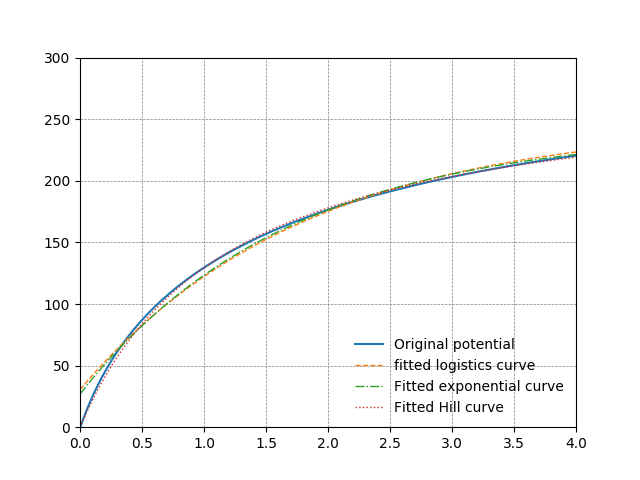
\includegraphics[width=\textwidth]{figures/Appendix/C_fit_NB_lim.png}
    \caption{4,000 timesteps}
    \label{fig:C_fit_NB_lim}
  \end{subfigure}
  \label{fig:Pot_noPH}
  \caption{Curve fitting using a generalized logistic function, Hall function, and exponential function of the potential of the MMO spacecraft without booms}
\end{figure}
\end{center}

\begin{center}
\begin{figure}[H]
  \begin{subfigure}[b]{0.61\textwidth}
    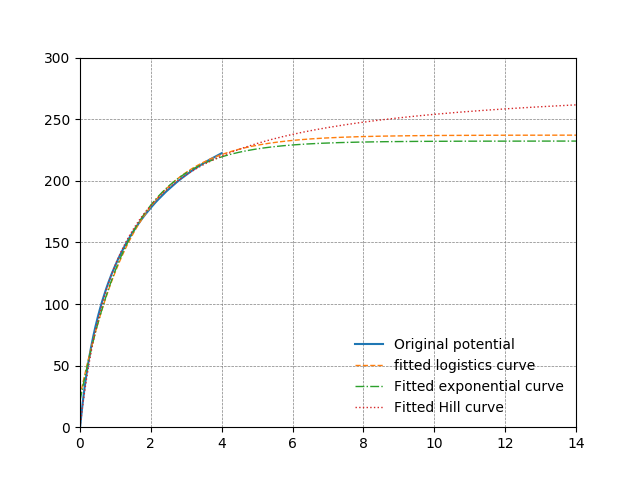
\includegraphics[width=\textwidth]{figures/Appendix/C_fit_WB.png}
    \caption{14,000 timesteps}
    \label{fig:C_fit_NB}
  \end{subfigure}
  \hfill
  \begin{subfigure}[b]{0.61\textwidth}
    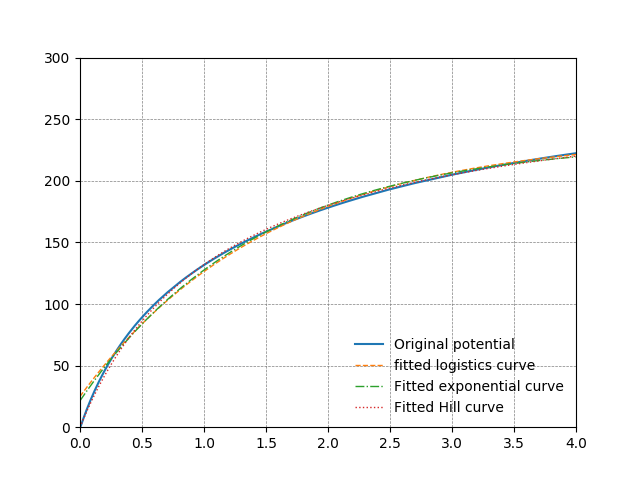
\includegraphics[width=\textwidth]{figures/Appendix/C_fit_WB_lim.png}
    \caption{4,000 timesteps}
    \label{fig:C_fit_NB_lim}
  \end{subfigure}
  \label{fig:Pot_noPH}
  \caption{Curve fitting using a generalized logistic function, Hall function, and exponential function of the potential of the MMO spacecraft with booms}
\end{figure}
\end{center}


\begin{longlisting}
\inputminted[
frame=lines,
framesep=2mm,
fontsize=\small
]{Python}{noPH_polyfit.py}
\caption{Python script for optimizing curves fit to the timeseries plot of electric potential. The optimized curves are plotted forward in time past the total number of timesteps simulated using PINC in order to estimate the floating potential of the MMO when no photoemission is included.}
\label{lst:polyfit}
\end{longlisting}